\documentclass{beamer}
%\usepackage{beamerarticle}
\usepackage{heppennames}
\usepackage{hepnicenames}
\usepackage{graphicx} 
\usepackage{multirow}
\usepackage{amsbsy,amsmath,amssymb}
\usepackage{booktabs}
% ********** Styl prezentacji **********
\mode<presentation>
{
	\usetheme{Singapore}
  \setbeamercovered{transparent}
   \setbeamertemplate{footline}[frame number] 
  \setbeamertemplate{navigation symbols}{ 
  \insertslidenavigationsymbol
  \insertframenavigationsymbol
  \insertsubsectionnavigationsymbol
  \insertsectionnavigationsymbol
  \insertdocnavigationsymbol
  \insertbackfindforwardnavigationsymbol
  \hskip 0.3cm
  %\insertframenumber / \inserttotalframenumber  % <<< frame #
  %\insertpagenumber / \insertpresentationendpage % <<< page #
} 
}

\usepackage[english]{babel}
\usepackage[latin1]{inputenc}

% font definitions, try \usepackage{ae} instead of the following
% three lines if you don't like this look
\usepackage{mathptmx}
\usepackage[scaled=.90]{helvet}
\usepackage{courier}


\usepackage[T1]{fontenc}

\author{S. Poss for the CERN LCD group}
\institute[CERN]{CERN}

\subject{CLICCDR}
\AtBeginSection[]
{
\usebackgroundtemplate{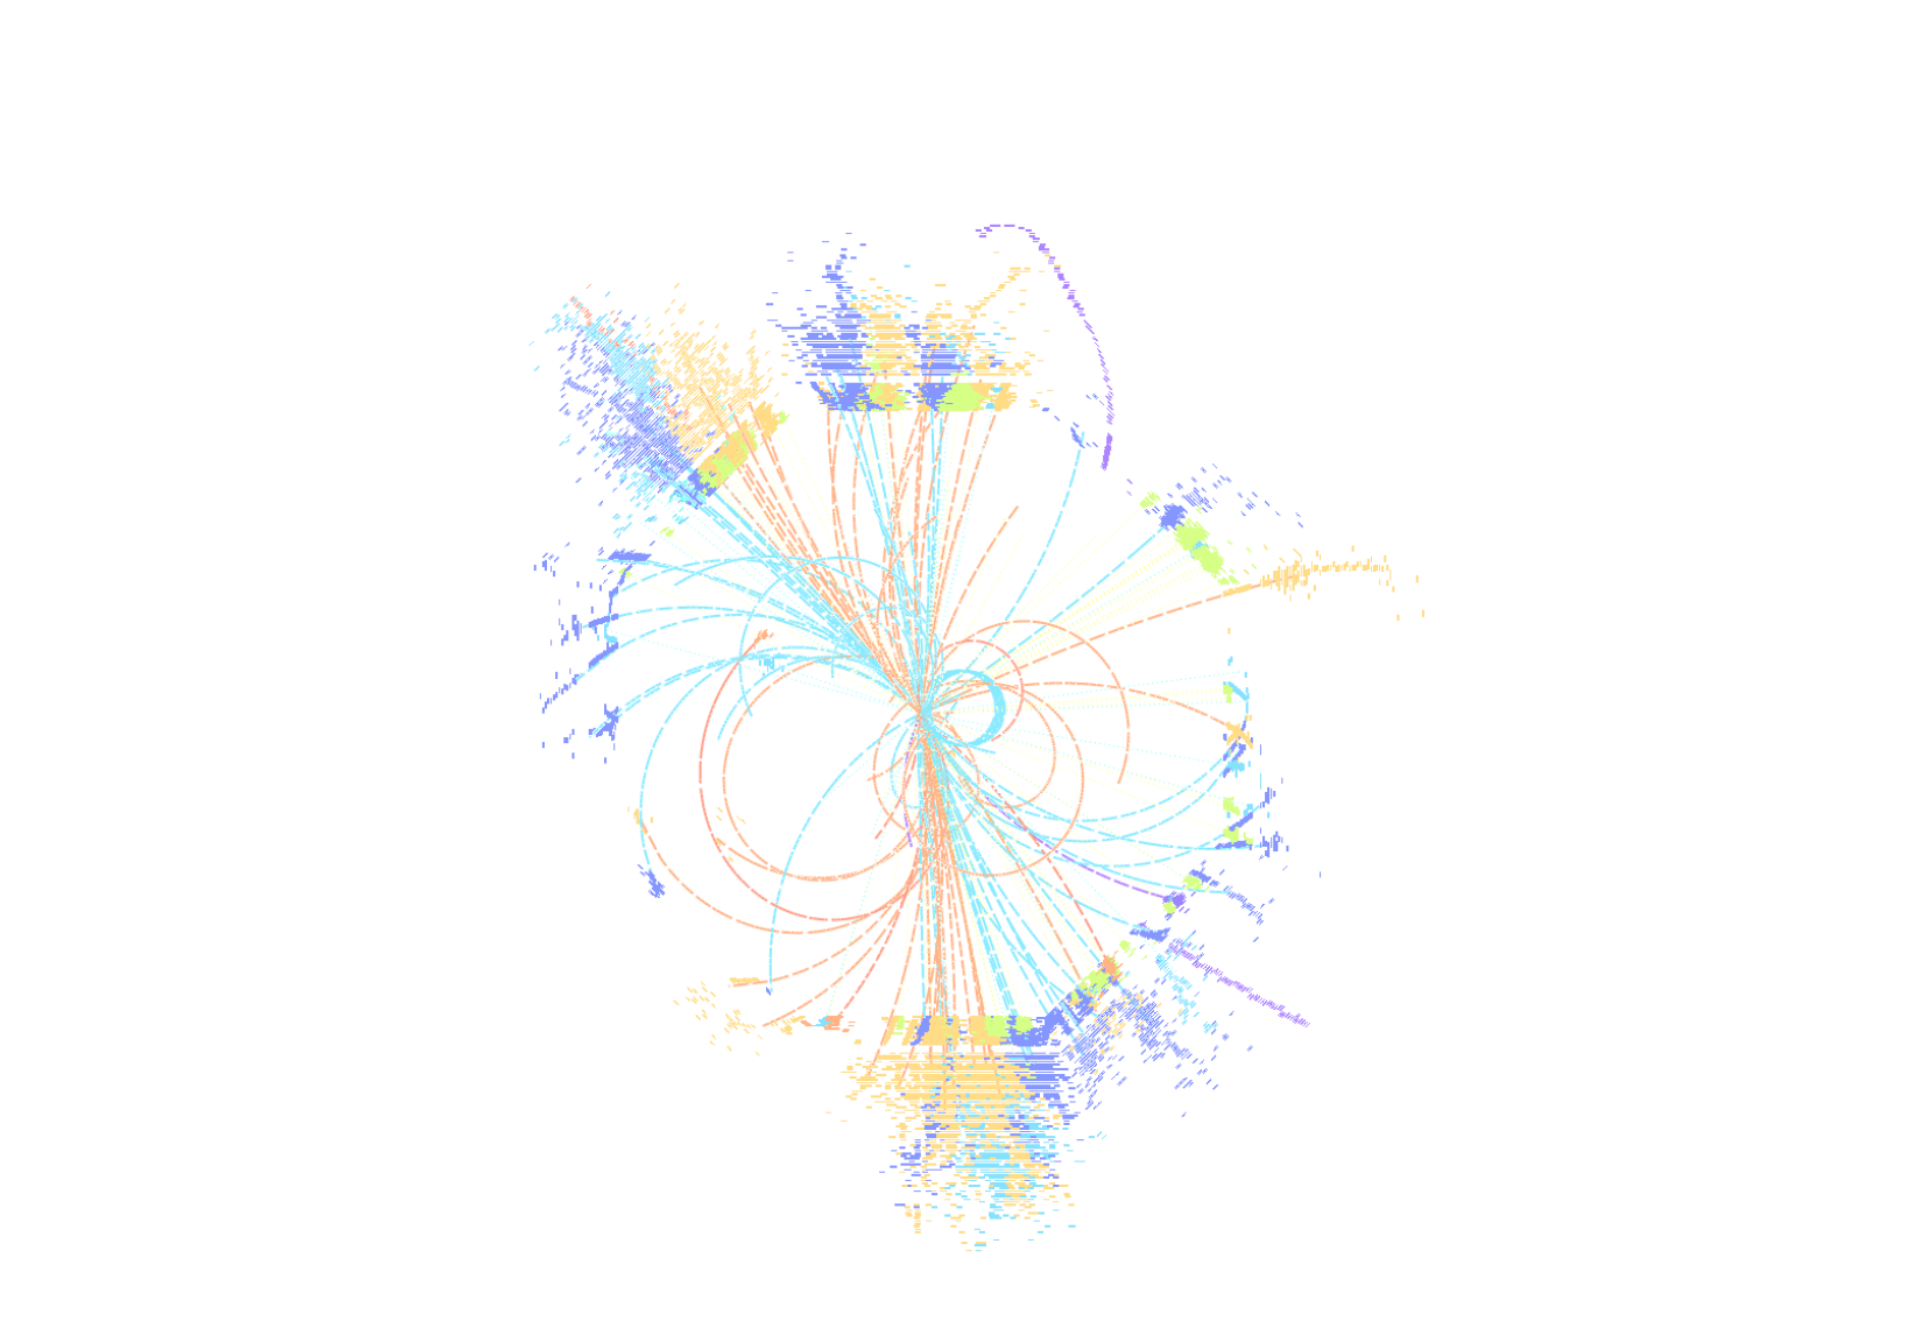
\includegraphics[width=\paperwidth]{background.png}}
	\begin{frame}<beamer>
		\frametitle{Outline}
		\tableofcontents[currentsection,currentsubsection]
	\end{frame}
}

\title[]{CLIC Physics CDR}
%%\subtitle{Our experience}

\date{\today}

\begin{document}

{
\usebackgroundtemplate{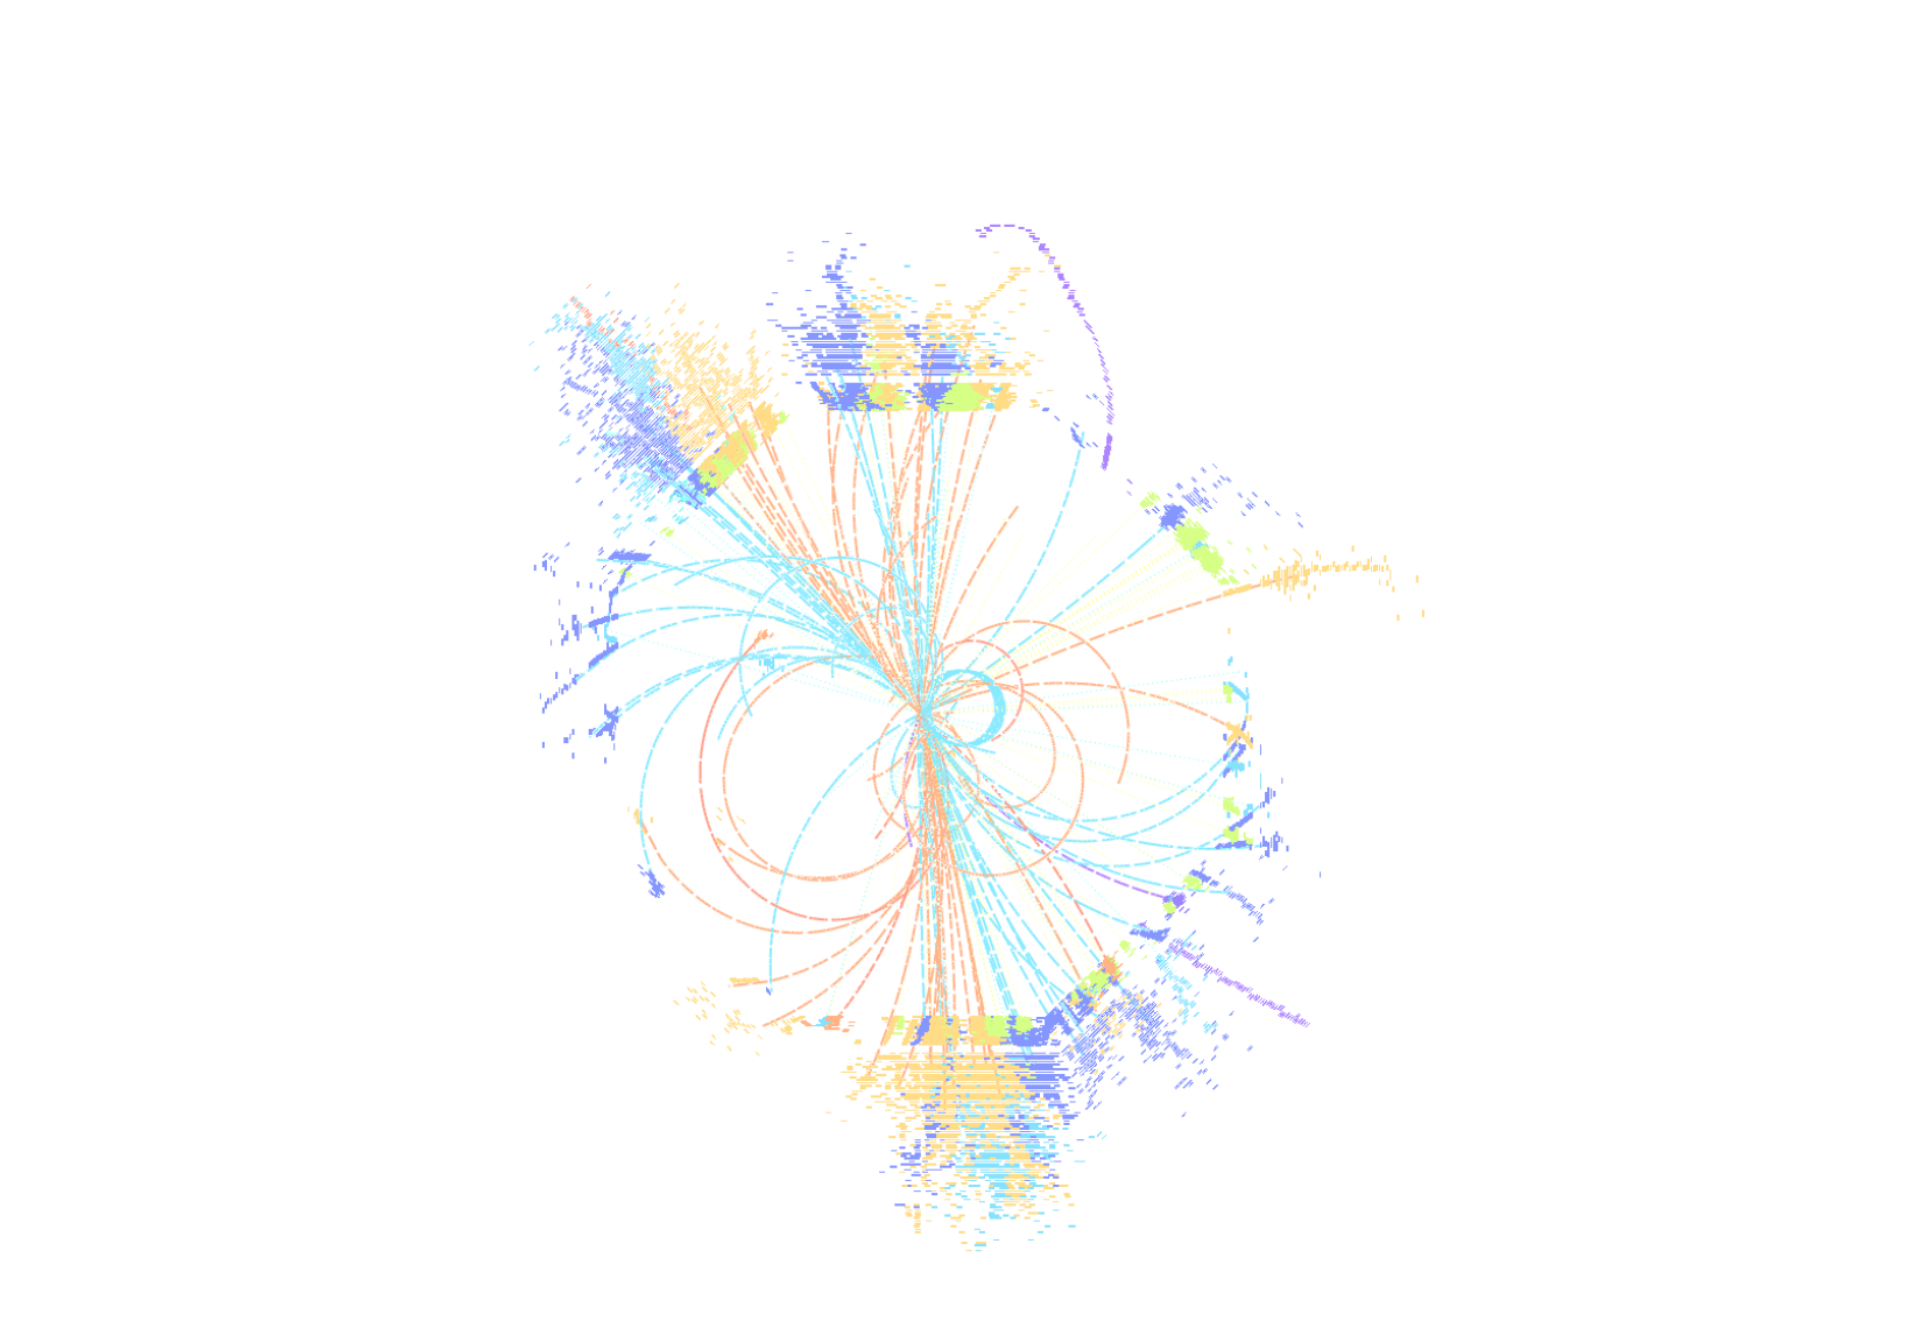
\includegraphics[width=\paperwidth]{background.png}}

\begin{frame}
	\titlepage
\end{frame}

\begin{frame}
\frametitle{Outline}
\tableofcontents
% You might wish to add the option [pausesections]
\end{frame}
}

\section{Motivations for a CLIC machine}%1slide

\section{Physics Potential}
\subsection{Higgs}%2slides
\subsection{SUSY}%2-3
\subsection{Other models and studies}%1slide

\section{Machine}
\subsection{Technology}%2-3slides
\subsection{MDI}%QD0 1slide
\subsection{Backgrounds}%2-3slides

\section{Detectors}
\subsection{Required performance}%1
\subsection{Generalities}%1
\subsection{Vertex detector design}%1-2
\subsection{Tracking: SiD}%1
\subsection{Tracking: ILD}%1
\subsection{ECAL design}%1
\subsection{HCAL design}%1
\subsection{CALICE results}%2

\section{Physics Results}
\subsection{Dealing with backgrounds}%4
\subsection{Higgs}%2
\subsection{Squarks}%2
\subsection{Sleptons}%2
\subsection{Gauginos}%2
\subsection{Heavy Higgs}%2
\subsection{Top physics at 500GeV}%3

\section{Conclusion}
\subsection{Overview}%1-2
\subsection{Signatory list}%1

\appendix
\section{Software}
\subsection{Generation}
\subsection{Simulation}
\subsection{Reconstruction}
\subsection{ILCDIRAC}


\end{document}